\chapter{Technische Aspekte}
Das folgende Kapitel behandelt den technischen Vergleich zwischen Angular und React. Zunächst werden grundlegende Entwurfsmuster und Modelle erläutert, die relevant für die weiteren Betrachtungen sind. 
Das Kapitel dient als Vorbereitung auf die noch folgende Implementation (Kapitel \ref{implementation}), die dort relevanten Bestandteile der Frameworks werden hier erläutert. 

\section{Grundlegende Schnittstellen und Entwurfsmuster}
\subsection{Komponenten}
2004 erscheint im Blog des Entwicklers und Architekturspezialisten Martin Fowler ein Artikel mit dem Titel \glqq Inversion of Control Containers and the Dependency Injection pattern\grqq. In diesem Artikel beschreibt er unter Anderem das Entwurfsmuster Dependency Injection (DI) als präziseren Begriff für Inversion of Control. Die Erkenntnisse aus dieser Betrachtung definieren grundlegende Entwurfsmuster von Angular, die in den folgenden Abschnitten erläutert werden. React ist nicht so stark an diese Konzepte gebunden.

Komponenten sind in der Terminologie nicht eineindeutig. Martin Fowler beschreibt seine Einordnung wie folgt:

\glqq I use component to mean a glob of software that's intended to be used, without change, by an application that is out of the control of the writers of the component. By 'without change' I mean that the using application doesn't change the source code of the components, although they may alter the component's behavior by extending it in ways allowed by the component writers.\grqq\cite{Fowler_Components}

Mit diesem Ansatz können Komponenten in React und Angular ebenfalls betrachtet werden. Eine Komponente ist in sich abgeschlossen und sollte von außen nicht verändert werden. Das Verhalten lässt sich ändern: Eine Beispielkomponente bietet eine Tabelle zum Anzeigen von Daten. Von außen lässt sich die Komponente bezüglich der Spalten, Zeilen, Styles und Inhalten in einem definierten Rahmen beeinflussen. Das Ziel ist wiederverwendbare Funktionalitäten mit erleichterter Wartbarkeit zu realisieren.

\subsection{Dependency Injection}
Das Entwurfsmuster Dependency Injection liefert einen Teil der Erklärung bereits mit seinem Namen: Abhängigkeiten werden \glqq injiziert\grqq. Die Tabellenkomponente dient in Listing {\ref{lst:listing5}} als Beispiel.

\begin{listing}
\caption{Dependency Injection}
\label{lst:listing5}
\begin{minted}{ts}
class TableComponent {
    private finder: EntryFinder;

    constructor(){
        this.finder = new EntryFinderImpl();
    }

    public getFilteredData(filter: string): Entry[] {
        let allEntries: Entry[] = this.finder.getAllEntries();
        let filteredEntries: Entry[] = allEntries.filter(entry =>
            entry.matches(filter));
        return (filteredEntries);
    }
}
interface EntryFinder{
    findAll(): Entry[];
}
\end{minted}
\end{listing}

Das finder-Objekt liefert die benötigten Daten für die Tabelle. Damit muss sich die \inlinecode{getFilteredData}-Methode nicht die Beschaffung der Entry-Objekte kümmern, das liegt in der Implementation der \inlinecode{Finder}-Klasse. Mit einem Interface kann die Kapselung noch klarer gemacht werden, dennoch ist eine konkrete Implementation notwendig (siehe Konstruktor). Diese ändert sich, abhängig von der konkreten Speicherung unserer Daten, z.B. im JSON-Format oder als SQL-Datenbank. Die Komponente ist also idealerweise nur vom Interface abhängig.

\subsection{Flux}
Flux ist ein von Facebook im Zusammenhang mit React entwickeltes Architekturmuster zum Management des Anwendungs-Zustands. Es berücksichtigt den unidirektionalen Datenfluss in React-Applikationen. Flux besteht aus 4 Teilen (siehe Abbildung \ref{fig:flux}).

\begin{figure}
  \centering
  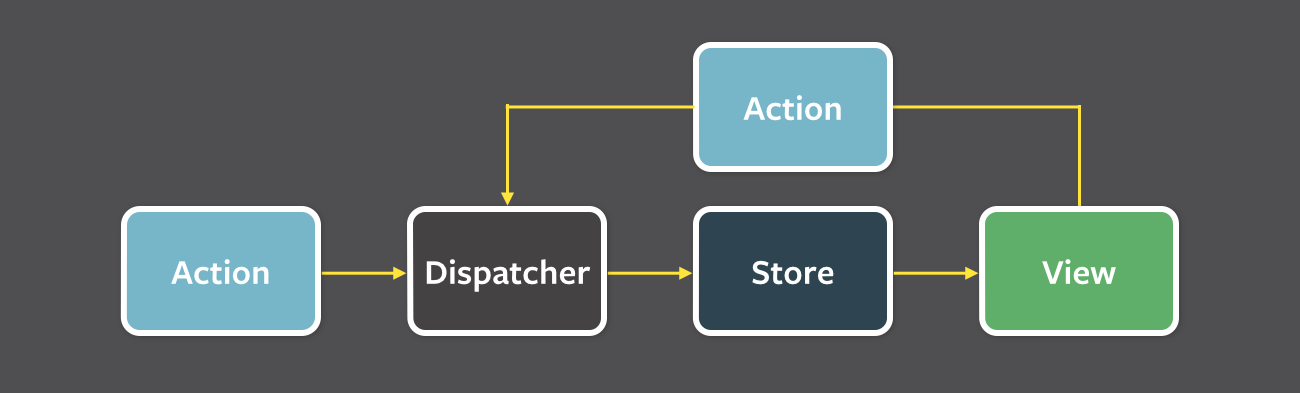
\includegraphics[scale=0.32]{Grafiken/flux.png}
  \quelle{https://facebook.github.io/flux/docs/in-depth-overview}
  \caption{Datenfluss mit Flux}
  \label{fig:flux}
\end{figure}

Der Store hält den für das Frontend relevanten anwendungsübergreifenden State. Die Views erhalten aus diesem Store ihre notwendigen Daten. Durch vom Nutzer angestoßene Änderungen in der View stößt diese Actions an, die der Dispatcher entgegen nimmt. Der Dispatcher veranlasst dann die Änderung des globalen States im Store.\cite{Flux_Concepts}

\subsection{Document Object Model}
Das Document Object Model, kurz DOM, ist eine API, die den Zugriff und die Manipulation von HTML- und XML-Dokumenten erlaubt. Aus diesen Dokumenten lässt sich eine Baumstruktur ableiten.

Browser verarbeiten HTML-Dokumente in eine solche Struktur, der DOM repräsentiert den aktuellen Zustand der gezeigten Seite. Dynamische Änderungen der Seite, die mittels JavaScript umgesetzt werden, sind einfache Veränderungen des DOM über die Schnittstelle -- beispielsweise mit den Funktionen \inlinecode{getElementById(...)} oder \inlinecode{removeChild(...)}.

\subsubsection{Virtual DOM}
React verwendet einen virtuellen DOM als Repräsentation des aktuellen Zustandes einer Komponente (siehe Abbildung \ref{fig:reactdom}). Ändern sich dargestellte Werte oder Elemente, so muss der DOM neu aufgebaut und dargestellt (gerendert) werden. Gerade bei kleineren Änderungen ist es aber nicht nötig, den gesamten DOM neu zu rendern. Der virtuelle DOM wird mit dem echten DOM abgeglichen, daraufhin werden nur die veränderten Elemente und Kindelemente neu gerendert\cite{VirtualDOM}. Mehr dazu im Abschnitt \ref{ssec:reconciliation}.

\begin{figure}
  \centering
  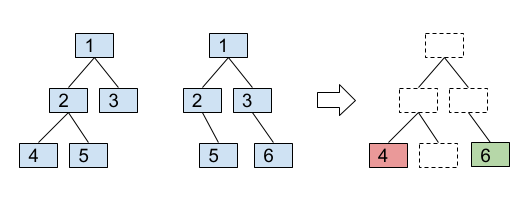
\includegraphics[scale=0.7]{Grafiken/reactvdom.png}
  \quelle{https://tinyurl.com/yyxtx766}
  \caption{Reacts Virtual DOM}
  \label{fig:reactdom}
\end{figure}

\section{Angular}
\subsection{Komponenten und Direktiven}
Angular-Applikationen besitzen mindestens eine Komponente. Diese besteht aus einer Klasse, die Daten und Programmlogik beinhaltet. Nach dem MVVM-Entwurfsmuster kann diese Klasse als das ViewModel bezeichnet werden. Die dazugehörige View ist ein HTML-Template, in welchem Daten für den Nutzer aufbereitet und dargestellt werden. Optional sind dazugehörige CSS-Styles, die bevorzugt in einem eigenen Stylesheet definiert werden. Komponenten beschreiben nur die Präsentation von Daten. Der Zugriff auf die Daten selbst sollte immer über einen Service stattfinden. Dadurch bleibt die Komponente unabhängig und einfacher testbar, etwa mit Mock-Up-Daten.

Listing \ref{lst:listing6} zeigt, wie die Klasse mit einem Dekorator\footnote{siehe: www.typescriptlang.org/docs/handbook/decorators.html} versehen wird, der für Angular notwendige Metadaten bereitstellt.

\begin{listing}
\caption{Component-Dekorator}
\label{lst:listing6}
\begin{minted}{typescript}
@Component({
    selector: 'app-example',
    templateUrl: './example.component.html',
    styleUrls: ['./example.component.css'],
    providers: [ ExampleService ],
})
export class ExampleComponent {
    /* ... */
}
\end{minted}
\end{listing}

Über den Dekorator können noch weitere Optionen angegeben werden. So lässt sich die Variante der Change Detection (siehe \ref{ssec:change_detection}) deklarieren, HTML und CSS als Strings auch direkt angegeben und zu injizierende Klassen definiert werden, die dann der Komponente und den Kindelementen über Dependency Injection zur Verfügung stehen.\cite{AngularConcepts}\cite{ComponentDecorator}

Direktiven definieren Programmlogik ohne eine dazugehörige View. Komponenten sind damit ebenfalls Direktiven, allerdings mit dazugehörigen Templates, die im DOM sichtbar sind. Ein Beispiel für Direktiven sind \inlinecode{ngFor} und \inlinecode{ngIf}. Erstere iteriert über iterierbare Objekte wie Arrays und gibt für jedes enthaltene Element wiederum HTML-Elemente zurück, die Zweite zeigt das Element abhängig von einer Bedingung.

\begin{listing}
\caption{ngFor und ngIf}
\label{lst:listing7}
\begin{minted}{html+ng2}
<span *ngFor="let number of numbers"> {{ number}} </span>

<!-- erzeugt ... -->
<span> 1 </span>
<span> 2 </span>
<span> 3 </span>

<!-- order-details erscheint nur im DOM, 
     wenn isPlanned wahr ist -->
<order-details *ngIf="order.isPlanned"></order-details->
\end{minted}
\end{listing}

Komponenten können miteinander kommunizieren: Eigenschaften werden dazu mit einem Input- oder Output-Dekorator versehen. Inputs sind dabei beliebige Objekte, im folgenden Beispiel eine Movie-Objekt, das relevante Daten zu einem Film enthält. Outputs sind Event-Emitter, über die ein Handler registriert werden kann. Dieser erhält dann den definierten Wert. Bei Verwendung der Komponente werden Klammern zur Bindung der jeweiligen Objekte verwendet, eckige für Input, runde für Output.

\begin{listing}
\caption{In- und Output in Angular-Komponenten}
\label{lst:listing8}
\begin{minted}{ts}
// movie-list.component.html
<movie-card [movie]="movie" (selected)="onSelected($event)">
// movie-card.component.ts
class MovieCardComponent {
    @Input()  movie: Movie;
    @Output() selected = new EventEmitter<number>();
    /* ... */
    public selected(): void {
        this.selected.emit(this.movie.id);
    }
}
// movie-list.component.ts
class MovieListComponent {
    public onSelected(event: number) { 
        // movieId verarbeiten ...
    }
}
\end{minted}
\end{listing}

\subsubsection{Lifecycle}
Der Lebenszyklus (Lifecycle) von Komponenten (und Direktiven) beginnt mit der Instanziierung der Komponenten-Klasse und dem Rendern der dazugehörigen View. Das gilt ebenso für alle Kindelemente. Die Change Detection erfasst Änderungen von Properties, die für die View relevant sind. Die Instanz wird gelöscht, wenn sie nicht weiter benötigt wird und die View aus dem DOM entfernt. Entwickler haben die Möglichkeit, in diesen Prozess einzugreifen, etwa um selbst Change Detection oder zusätzliche Aufräumarbeiten beim Löschen der Komponente zu initiieren. Das geschieht über Hooks, \inlinecode{ngOnInit()} wird beispielsweise direkt nach der Instanziierung der Komponente aufgerufen und eignet sich für das asynchrone Laden von Daten. Weitere Hooks sind z.B. \inlinecode{ngAfterViewInit()}, der Aufruf geschieht direkt nach der Initialisierung aller Views (auch Kindelemente) oder \inlinecode{ngOnDestroy()}, wird vor der Löschung der Komponente ausgeführt.\cite{AngularHooks}

\subsubsection{Services}
Als Services werden in Angular spezielle Klassen bezeichnet, die sich um die Bereitstellung von Daten kümmern oder Programmlogik kapseln, die nicht in Komponenten gehört. Häufig werden mit Services Anwendungsdaten über das HTTP-Protocol von einem Server abgerufen, dort verändert oder abgespeichert. Angular liefert eine eigene HTTP API mit, welche diesen Zugriff ermöglicht. Ein Beispiel findet sich später in der Angular-Implementation (\ref{sssec:impl_services}).
Ein anderes Beispiel wäre ein Service zum Loggen von definiertem Anwendungsverhalten, um etwa speziellen Zugriff zu dokumentieren oder die Entwicklung zu unterstützen.

Service-Klassen werden wie Komponenten und Direktiven mit einem Dekorator versehen und damit als solche markiert. Dieser nimmt lediglich eine Option entgegen: \inlinecode{providedIn}. Diese nimmt einen Injector für die Dependency Injection entgegen, üblicherweise 'root'. Damit steht der Service allen Komponenten zur Verfügung und kann wie soeben beschrieben über den Konstruktor eingebunden werden. Soll der Service nur in ausgewählten Modulen oder Komponenten nutzbar sein, dann muss der Service dort im Dekorator unter der Option \inlinecode{providers} deklariert werden. Services können wiederum andere Services einbinden.\cite{Services}

\subsubsection{Pipes}\label{ssec:pipes}
Angular-Pipes basieren auf dem bekannten Prinzip von Pipes, welches ursprünglich für das Unix-Betriebssystem entwickelt wurde. In diesem Sinne ist eine Pipe(line) die Verbindung zwischen zwei datenverarbeitenden Prozessen, die Ausgabe des ersten wird zur Eingabe des zweiten Prozesses. Angular setzt auf dieses Grundprinzip. Mit Pipes sind allerdings transformierende Operationen gemeint, nach dem ursprünglichen Modell also der zweite Prozess selbst.

Pipes definieren eine \inlinecode{transform}-Funktion, die Parameter entgegen nimmt und einen transformierten Wert zurückgibt. Angular besitzt vordefinierte Pipes, unter anderem eine \inlinecode{DatePipe} zur Umwandlung von Daten in das lokale Zeitformat, eine \inlinecode{CurrencyPipe} zur Umwandlung von Zahlen in einen String mit der lokalen Währung oder eine \inlinecode{UpperCasePipe} zur Umwandlung von Text in Großbuchstaben. Pipes werden üblicherweise in Templates verwendet\cite{AngularPipes}:

\mintinline{html+ng2}{
<span>Auftragsdatum: {{ orderDate | date }}</span>
}

Komplexer ist die \inlinecode{AsyncPipe}, 
diese gibt den letzten emittierten Wert von Observables\footnote{siehe: https://rxjs-dev.firebaseapp.com/guide/observable} 
oder Promises\footnote{siehe: https://developer.mozilla.org/de/docs/Web/JavaScript/Reference/Global\_Objects/Promise} 
durch eine Subscription\footnote{siehe: https://rxjs-dev.firebaseapp.com/guide/subscription} zurück. 
Ein häufiger Anwendungsfall ist die Einbindung von Daten aus asynchronen Operationen (Listing \ref{lst:listing7}).\cite{AsyncPipe}

\begin{listing}
\caption{AsyncPipe}
\label{lst:listing9}
\begin{minted}{html+ng2}
<div *ngIf="orders$ | async as orders; else #noResults">
    <!-- Das Objekt 'orders' kann verwendet werden ... -->
</div>
<ng-template #noResults>
    <span> Keine Aufträge gefunden. </span>
</ng-template>
\end{minted}
\end{listing}

\subsection{Modules}
Angular-Applikationen werden mit \inlinecode{NgModules} modular aufgebaut. Module fassen Komponenten, Services und sonstigen Quelltext zusammen, die ein gemeinsames Feature abbilden oder auf andere Art und Weise zusammen gehören. Beispiele: Das \inlinecode{BrowserModule} stellt die notwendige Infrastruktur bereit, um Angular Applikationen im Browser starten zu können und ist damit Standard. Um Direktiven wie \inlinecode{ngIf} oder \inlinecode{ngFor} zu nutzen, muss das \inlinecode{CommonModule} importiert werden. Services benötigen das \inlinecode{HttpClientModule} zur Kommunikation mit Servern. Die zwei zuerst genannten Module werden für alle Komponenten benötigt und daher direkt im \inlinecode{app.module} importiert. Jede Anwendung deklariert mindestens dieses Modul. Module sind ebenfalls Klassen, werden aber ausschließlich durch den \inlinecode{NgModule}-Dekorator beschrieben (Listing \ref{lst:listing10}).\cite{NgModule}

\begin{listing}
\caption{NgModule}
\label{lst:listing10}
\begin{minted}{typescript}
@NgModule({
  declarations: [
    // Komponenten, Direktiven und Pipes,
    // die zu diesem Modul gehören
    ExampleComponent,
    ExampleDirective,
    ExamplePipe
  ],
  imports: [ 
    // Andere Module, die den deklarierten Be-
    // standteilen des Moduls zur Verfügung stehen
    BrowserModule,
    SomeOtherModule
  ],
  providers: [
    // Mittels DI injizierbare Objekte
    ExampleService
  ],
  exports: [
    // Bestandteile des Moduls, die beim Import
    // des Moduls bereitgestellt werden
    ExampleComponent
  ]
})
export class ExampleModule { }
\end{minted}
\end{listing}

\subsection{Dependency Injection}
Es gibt verschiedene Varianten der Dependency Injection, die von Angular verwendete Variante nennt sich Constructor Injection (Listing \ref{lst:listing11}). Die Objekte, zu welchen eine Abhängigkeit der Komponente besteht, werden dem Konstruktor übergeben. In der Regel sind abhängige Objekte Services, es können allerdings auch Funktionen oder Werte injiziert werden.

\begin{listing}
\caption{Verwendung von Services über Constructor Injection}
\label{lst:listing11}
\begin{minted}{typescript}
export class ExampleComponent {
    constructor(
        private finderService: EntryFinderService,
        public printService: PrinterService
    ) {}
}
\end{minted}
\end{listing}

Angular initialisiert einen \inlinecode{Injector}, der einen Container mit Dependency-Instanzen verwaltet. Über einen Provider wird dem Injektor mitgeteilt, wie eine Instanz erzeugt wird, üblicherweise sind das die Klassen der Services. Wenn Angular eine neue Komponente erzeugt, dann wird überprüft, welche Abhängigkeiten bestehen. Gibt es Abhängigkeiten ohne bestehende Instanz, dann werden diese erzeugt und der Komponente zur Verfügung gestellt. Erkennbar ist, dass DI auf dem Singleton-Entwurfsmuster aufbaut. Damit werden Inkonsistenz und redundante Objekte vermieden.
Angulars DI bietet viele Möglichkeiten, die hier nicht in die Tiefe behandelt werden\footnote{siehe: https://angular.io/guide/dependency-injection}. Relevant für die noch folgende Implementation ist die einfache Injektion von Services.\cite{ServiceDI}

\subsection{Change Detection}\label{ssec:change_detection}
Change Detection versucht Veränderungen des Anwendungszustandes zu erkennen und die View entsprechend zu updaten. In Angular geschieht das automatisch. Wird in einem Template ein Verweis auf Daten erzeugt (z.B. \inlinecode{\{\{user.name\}\}}) -- sogenannte \textit{Bindings} -- dann beobachtet Angular dieses Element und prüft auf Wertveränderungen: Change Detection. Ausgelöst durch Browser-Events (Mausklick, Tastatureingaben), HTTP-Anfragen oder spezielle Funktionen wie \inlinecode{setInterval} oder \inlinecode{setInterval} wird der komplette Komponentenbaum abgetastet (siehe Abbildung \ref{fig:comp_tree})

\begin{figure}
    \centering
    \begin{forest}
        changed/.style={fill=red!50, rounded corners, text=black},
        for tree={fill=black!50, text=white, rounded corners}
            [Comp Root
                    [Comp A
                            [Comp C]
                            [Comp D]]
                    [Comp B
                            [Comp E
                                    [Comp G, changed]]
                            [Comp F]]
            ]
    \end{forest}
    \caption{Komponentenbaum mit Veränderung in Komponente G}
    \label{fig:comp_tree}
\end{figure}

Diese Variante kostet unter Umständen zu viel Zeit. Als Alternative kann daher die Strategie auf \inlinecode{onPush} geändert werden. Mit onPush markierte Komponenten werden nicht automatisch überprüft. Change Detection findet hier nur statt, wenn:

\begin{itemize}
    \item Eingabewerte verändert werden, z.B. die Datenquelle einer Tabellenkomponente
    \item die Komponente oder Kindkomponenten spezielle Events auslösen, z.B. ein Button wird angeklickt
    \item sie manuell ausgelöst wird
    \item in Templates referenzierte Observables neue Werte ausliefern
\end{itemize}

Die Change Detection sollte vor allem bei größeren Anwendungen mit vielen Komponenten beachtet werden. Ein Wechsel auf die onPush-Strategie verbessert gegebenenfalls die Performance.\cite{ChangeDetection}

\subsection{State-Management}

State-Management kann in Angular auf verschiedenen Wegen umgesetzt werden. Über Input-Attribute kann übergreifender State im Komponentenbaum verteilt und bei Änderung mit Output-Events nach oben gereicht werden. Für komplexere Anwendungen gibt es besser Ansätze: Redux\footnote{siehe: https://redux.js.org/}, eine auf Flux basierende Bibliothek, oder Observable Data Services\footnote{siehe: https://coryrylan.com/blog/angular-observable-data-services}.

\subsection{Projektarchitektur}
Angular gibt durch die beschriebenen Features Empfehlungen über den Aufbau der damit gebauten Anwendung und zu verwendende Entwurfsmuster ab. Die Dokumentation stützt sich auf diese Prinzipien, auch wenn sie nicht zwangsläufig befolgt werden müssen, um eine funktionsfähige Anwendung zu entwickeln. Angular empfiehlt, den Code in möglichst kleine Komponenten aufzuteilen. Jede Komponente übernimmt möglichst nur eine Aufgabe. Komponenten die zu dem gleichen Teilbereich gehören werden als Modul zusammengefasst.

Einzelne Komponenten lassen sich mit dem MVVM-Entwurfsmuster vergleichen. Das Model sind einfache Klassen und Interfaces, welche die Daten der Anwendung modellieren, z.B. Nutzer, Auftrag oder Rezept. Models enthalten keine Programmlogik, die Ausnahme bildet die Validierung der Daten. Services werden von Komponenten genutzt, um auf Models zuzugreifen. Komponenten vereinen die View und das ViewModel aus MVVM: Die HTML-Templates mit dazugehörigen Styles beschreiben die Darstellung von Daten für den Endnutzer. Die TypeScript-Klassen sind das ViewModel, stehen also zwischen dem Model und der View. Die View greift auf das ViewModel zu und kann es gegebenenfalls modifizieren, etwa durch Nutzereingaben (Zweiseitige Datenbindung). Das Model wird vom ViewModel abgerufen und ebenfalls modifiziert, sollten die Änderungen in der View das erfordern.

\begin{figure}
  \centering
  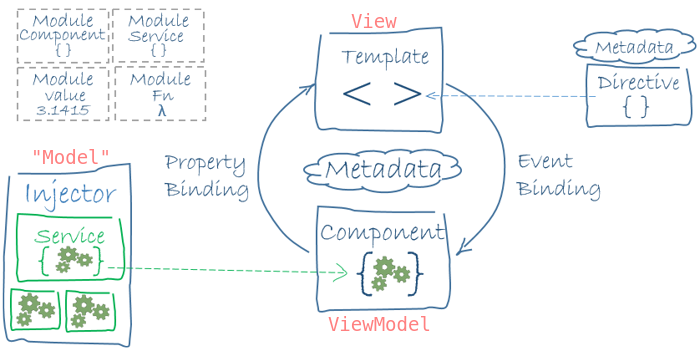
\includegraphics[scale=0.6]{Grafiken/MVW.png}
  \quelle{https://angular.io/guide/architecture}
  \caption{Angular Architektur}
\end{figure}

Entwickler haben die Freiheit, wie konsequent sie die Trennung vornehmen. Services passen nur bedingt in das MVVM-Entwurfsmuster, sie stehen zwischen Model und ViewModel. Angulars Nähe zu MVVM ist erkennbar und hilft beim Verständnis. Am Ende definiert das Framework aber eigene Prinzipien und gibt dem Entwickler genügend Spielraum, wie er Programmlogik strukturieren möchte.\cite{MVVM}\cite{AngularArchitecture}

\section{React}
\subsection{Komponenten}
Die Grundeinheiten sind die React Elements. Diese können gängige DOM-Tags:

\mintinline{jsx}{const element = <div />;}

oder deklarierte Komponenten enthalten:

\mintinline{jsx}{const helloMax = <Greeting name="Max">;}

\subsubsection{Funktions- und Klassenkomponenten}
Es gibt mehrere Möglichkeiten in React, Komponenten zu deklarieren. Das Konzept ähnelt Funktionen: Sie erhalten beliebigen Input über die sogenannten \inlinecode{props} und geben eine Beschreibung dessen, was auf dem Bildschirm angezeigt werden soll als React-Objekte zurück. In Listing \ref{lst:listing12} werden zwei prinzipiell äquivalente Varianten gezeigt\cite{ComponentsProps}. Komponenten können wie React Elements andere Komponenten enthalten.

\begin{listing}
\caption{Funktions- und Klassenkomponenten in React}
\label{lst:listing12}
\begin{minted}{jsx}
// Komponente als Funktion
function Greeting(props) {
    return <h1>Guten Tag {props.name}!</h1>;
}

// Komponente als Klasse, implementiert die render-Funktion
class Greeting extends React.Component {
    render() {
        return <h1>Guten Tag {props.name}!</h1>;
    }
}
\end{minted}
\end{listing}

Darüber hinaus gibt es Higher-Order-Components\footnote{siehe: https://reactjs.org/docs/higher-order-components.html}. Diese verarbeiten Komponenten als Argumente und geben wiederum Komponenten zurück. Mit Higher-Order-Components lässt sich Logik extrahieren und wiederverwenden. Beispiel: Zwei Komponenten zeigen unterschiedliche Medientypen (z.B. Videos und Bilder) in einer Listenansicht an. Beide Komponenten abonnieren eine Datenquelle, verändern ihren State wenn sich die Datenquelle ändert und deabonnieren die Datenquelle zum Ende ihres Lebenszyklus. Diese gemeinsame Funktionalität lässt sich in einen HoC extrahieren. HoC sind jedoch keine eigene Klasse aus der React-Bibliothek, sondern nur ein empfohlenes Pattern der Entwickler.

\subsubsection{UI-State und Lifecycle}
Nicht alle Komponenten liefern nur statische Inhalte abhängig von Props. Um komplexere Komponenten zu erstellen benötigen Komponenten eine State. Dieser State beinhaltet definierte Werte und existiert solange wie die Komponente selbst. Ein einfaches Beispiel ist ein Timer: Hier muss die abgelaufene Zeit gespeichert werden, sonst bleibt der Timer beim initialen Wert stehen. React liefert für Klassenkomponenten das Attribut \inlinecode{state} und die Funktion \inlinecode{setState} mit. 

React besitzt ebenfalls Lifecycle-Hooks. \inlinecode{componentWillMount} und \inlinecode{componentWillUnmount} entsprechen z.B. Angulars \inlinecode{ngOnInit} und \inlinecode{ngOnDestroy} und dienen zur Vorbereitung der View oder Aufräumen zur Vermeidung von Memory-Leaks (Listing \ref{lst:listing13}).
 
\begin{listing}
\caption{Lifecycle-Methoden in React}
\label{lst:listing13}
\begin{minted}{jsx}
class Timer extends React.Component {
    constructor(props) {
        super(props);
        this.state = { time: 0 };
    }

    componentDidMount() {
        this.timerInterval = setInterval(
            () => this.setState({
                    time: this.state.time + 1()
             });
            1000
        );
    }

    componentWillUnmount() {
        clearInterval(this.timerInterval);
    }

    render() {
        return (
            <div>
            <h1>Timer</h1>
            <h2>Es sind {this.state.time}s vergangen.</h2>
            </div>
        );
    }
}
\end{minted}
\end{listing}

\subsubsection{Hooks}
Hooks sind ein relativ neues Feature in React, sie wurden mit Version 16.8 Anfang 2019 eingeführt. Sie versuchen einige Probleme zu lösen, die besonders mit Klassenkomponenten verursacht werden: 

\begin{itemize}
    \item Wrapper Hell: Schachtelung von Komponenten ermöglicht die Wiederverwendung von Logik. Das führt zu Unübersichtlichkeit, Debugging wird erschwert
    \item Klassenkomponenten sind durch viel Boilerplate schwer zu lesen und überladen
    \item Klassenkomponenten sind nicht intuitiv. \inlinecode{this} verhält sich in JavaScript anders, Memberfunktionen müssen mit \inlinecode{bind()} im Konstruktor registriert werden\cite{HooksYoutube}
\end{itemize}

Hooks lösen die Probleme mit Klassenkomponenten durch eine lesbare und funktionale API, mit Custom Hooks lässt sich mehrfach benötigte Logik extrahieren.
Die zwei wichtigsten Hooks sind \inlinecode{useState} und \inlinecode{useEffect}, ein Beispiel ist in Listing \ref{lst:listing14} zu sehen.

\begin{listing}
\caption{React-Hooks useState und useEffect}
\label{lst:listing14}
\begin{minted}{jsx}
function Greeting() {
    // Status und Setter definieren, Hook setzt initialen Status
    const [userName, setUserName] = useState('Max');
    const [timeOnline, setTimeOnline] = useState(0);

    // fasst Lifecycle-Methoden zusammen, die zurückgegebene Funktion wird beim Clean-up ausgeführt
    useEffect(() => { 
        function handleStatusChange(status) {
            setUserName(status.userName)
            setTimeOnline(status.onlineTime);    
        }

        UserAPI.subscribeToUserStatus(handleStatusChange);

        return function cleanup() {
            UserAPI.unsubscribeFromUserStatus(handleStatusChange);
        }
    );

    return (
        <span>
            {name} ist seit {timeOnline} Minuten online!
        </span>
    );
}
\end{minted}
\end{listing}

\subsection{Reconciliation}\label{ssec:reconciliation}
Reconciliation ist der Change Detection Algorithmus von React. Ausgelöst wird der Algorithmus durch die Veränderung des Status über Hooks oder \inlinecode{setState}. Jeder Aufruf der \inlinecode{render()} Funktion liefert einen neuen Baum mit React Elementen, der nun möglichst effektiv verarbeitet werden muss. React vergleicht zunächst die \inlinecode{root}-Knoten, sind sie unterschiedlich, dann wird der komplette Baum neu aufgebaut. Sind die Elemente gleich, dann werden als Nächstes die Attribute verglichen. React iteriert im Anschluss über die Kindelemente. Einfügungen sind problematisch, da für den Algorithmus aufgrund der einfachen Iteration nicht feststellbar ist, ob ein Unterbaum intakt bleiben kann. Umgehen lässt sich das Problem mit Keys. Über das gleichnamige Attribut werden die Kindelemente verglichen, einfache Verschiebungen im Unterbaum werden so erkannt. Die ID wird in der Regel von der Objekt-ID abgeleitet: 

\mintinline{jsx}{<li key={user.id}>{user.name}</li>}

Reconciliation ist eng verzahnt mit dem Lebenszyklus von Komponenten. Der Unterschied zu Angular liegt besonders darin, das Komponenten inklusive State komplett gelöscht und neu gerendert werden, wenn sich der Status ändert, während Angular lediglich die Bindings mit dem neuen Wert anpasst.\cite{Reconciliation}

\subsection{State-Management}
State Management in React ist eine komplexere Aufgabe. Der bereits betrachtete UI-State bezieht sich nur auf eine Komponente und ist beim nächsten Rendern verloren. Darüber hinaus können Komponenten nicht miteinander kommunizieren. Beispiel: Eine Komponente zeigt den aktuell angemeldeten Nutzer und einen Statustext an. In einer anderen Komponente gibt es ein Formular, mit dem Name und Statustext verändert werden können. Beide Komponenten benötigen den initialen State, der Formulareintrag in Komponente 2 ändert zwar dort die Werte, Komponente 1 verbleibt aber im ursprünglichen Zustand. Eine Lösungsmöglichkeit besteht darin, neben dem User-Objekt eine Callback-Funktion aus der Elternkomponente durch den Baum zu geben. Komponente 2 übergibt die Änderungen an diese Funktion, welche dann das User-Objekt modifiziert. Die nachfolgende Change Detection aktualisiert dann den neuen State in beiden Komponenten. Diese Methode ist zwar einfach, für umfangreiche Anwendungen mit komplexeren States und Abhängigkeiten führt dieses Vorgehen schnell zu chaotischem Programmcode. 

Die von den React-Entwicklern vorgeschlagen Lösung ist das Flux-Entwurfsmuster. React besitzt mit der Context API\footnote{siehe: https://reactjs.org/docs/context.html} eine integrierte Lösung, um Daten mehreren Komponenten zur Verfügung zu stellen, ohne Props durch den ganzen Baum zu reichen. Damit lässt sich Flux implementieren. Redux ist wie bei Angular eine andere Möglichkeit. Eine weitere Alternative ist eine eigene Implementation von Dependency Injection und Services mit Observables. Egal worauf die Entscheidung fällt, für komplexere Anwendungen ist State-Management notwendig, React selbst bietet hier keine Lösungen an und überlässt dem Software-Architekten die Wahl. 

\subsection{Projektarchitektur}
React bricht im Gegensatz zu Angular mit klassischen MV*-Entwurfsmustern, die \textit{Separation Of Concerns} (dt. Trennung der Verantwortlichkeiten) als Zielstellung verfolgen. JSX vereint Logik und View, statt sie zu trennen. Separation of Concerns ist mit der richtigen Komposition von Komponenten trotzdem umsetzbar, lediglich die Herangehensweise verändert sich (Listing \ref{lst:listing16}).

Mit React lassen sich wiederverwendbare Bausteine entwickeln, die dann als Komposition verschachtelt werden können. React verfolgt damit das Ziel, die Menge an Programmcode weiter zu reduzieren\cite{ReactSoC}. Am Ende bleibt React eine Frontend-Bibliothek zur Generierung von HTML. Die Architektur der Anwendung bleibt dem Software-Architekten und die Einhaltung der definierten Regeln den ausführenden Entwicklern überlassen. React forciert anders als Angular keine Entwurfsmuster, das Entwicklerteam von Facebook gibt nur Empfehlungen ab.

\begin{listing}
\caption{Trennung von View und Logik durch Komposition}
\label{lst:listing16}
\begin{minted}{jsx}
class FetchEvents extends React.Component {
    /* Konstruktor und State ... */
    componentDidMount() {
        /* Aufrufe zur Backend-API ... */
    }
    /* View-Logik ... */
    render() {
        return this.props.children({ this.state.isLoading, this.state.events });
  }
}

class App extends React.Component {
    render (
        <FetchEvents>
        {({ isLoading, events }) => {
            if (isLoading) 
                return <p>Termine laden ...</p>;
            if (events) 
                return events.map(({ title }) => 
                    <p>Terminname: {title}</p>);
            else return null;
        }}
        </FetchEvents>
  );
}
\end{minted}
\end{listing}